\begin{Exercise}[title=Modélisation d'un haut-parleur]
		\begin{minipage}{.6\linewidth}
			On modélise la partie mécanique d’un haut-parleur à
			l’aide d’une masse $m$, se déplaçant horizontalement
			sans frottement le long de l’axe $(O,\vec{e_x})$. Cette masse,
            assimilée à un point matériel M, est reliée à un ressort de longueur
            à vide $l_0$ et de raideur $k$, ainsi qu’à un amortisseur fluide de
            constante $f$ . Elle est soumise	à une force $\vec{F(t)}$,
            imposée par le courant i(t) entrant dans le haut-parleur.
            On a : $F(t) = K i(t)\vec{e_x}$, avec $K$ une constante.
			On suppose que le courant $i(t)$ est sinusoïdal : $i(t) =
			I_m cos(\omega t)$.
			\emph{Données : $m= 10g$, $k= 15kN.m^{-1}$, $K=200N.A^{-1}$et $I_m=1A$}
		\end{minipage}\hspace*{0.05\linewidth}\begin{minipage}{.3\linewidth}
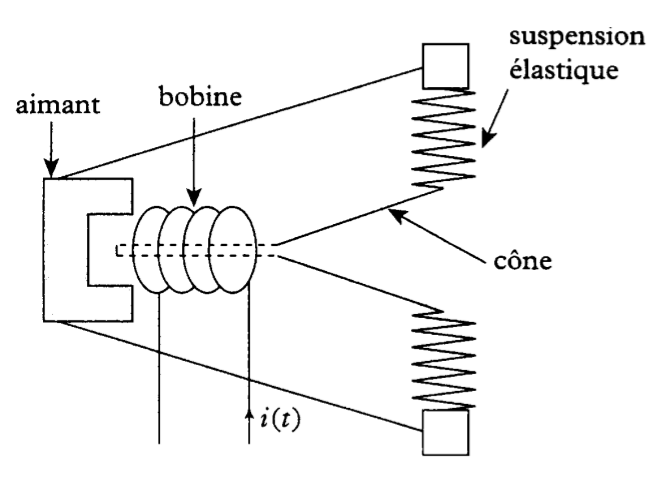
\includegraphics[width=\textwidth]{../fig/haut-parleur}
		\end{minipage}
	\Question Proposer un modèle mécanique équivalent.
	\Question Écrire l'équation différentielle vérifiée par la position de la masse $m$.
	\Question La normaliser. On veux $Q= \frac{1}{\sqrt{2}}$ pourquoi? Calculer alors la valeur du coefficient $f$
	\Question Déterminer  l'expression de la réponse forcée $x(t)$ et la mettre sous la forme $X_m \cos{\omega t+ \phi}$.\emph{On donne $\omega =$\SI{6280}{rad\per\s}}.
	\Question Tracer le diagramme de Bode correspondant, Déterminer la bande passante.
\end{Exercise}
\begin{Answer}
	\Question Ressort + amortisseur en parallèle.
	\Question $\ddot{x}+\frac{f}{m}\dot{x}+\frac{k}{m}x = \frac{K}{m}I_m \cos(\omega t)$
	\Question $\omega_0 = \sqrt{\frac{k}{m}}$ et $Q= \frac{\sqrt{km}}{f}$ AN : $f \simeq 17.3kg/s$
	\Question $\omega_0 = 1225 rad/s $ , $X_m=0.5 mm$ et $\phi = -2.86 rad$
	\Question $X_m(\omega_c) = \frac{KI_m}{m\omega_0}\frac{1}{\sqrt{1+\frac{\omega_c^4}{\omega_0^4}}}=\frac{X_m(max)}{\sqrt{2}} \Leftrightarrow  \omega_c =\omega_0$
\end{Answer}
